%% -*- coding: utf-8 -*-
\documentclass[12pt,pagesize,paper=192mm:108mm,landscape]{scrbook} 
%1920x1080 1280x720
\areaset[current]{192mm}{108mm}
\usepackage{calc}
\usepackage[T2A]{fontenc}
\usepackage[utf8]{inputenc}
\usepackage[english,russian]{babel}
\usepackage{microtype}
\usepackage{misccorr}
\usepackage{cmap}
%\usepackage[unicode=true]{hyperref}
\usepackage{graphicx}
\usepackage{amssymb}
\usepackage{amsmath}
%\usepackage{srcltx}
\usepackage{textcomp}
\usepackage{xspace}
%научные символы и смайлики \smiley \frownie
\usepackage{wasysym}
\usepackage{ccicons}
\begin{document}
\begin{titlepage}
  \vspace*{-0.5em}
  \begin{center}    
    % \hspace*{3em}
    % \begin{minipage}[t]{3em}
    %   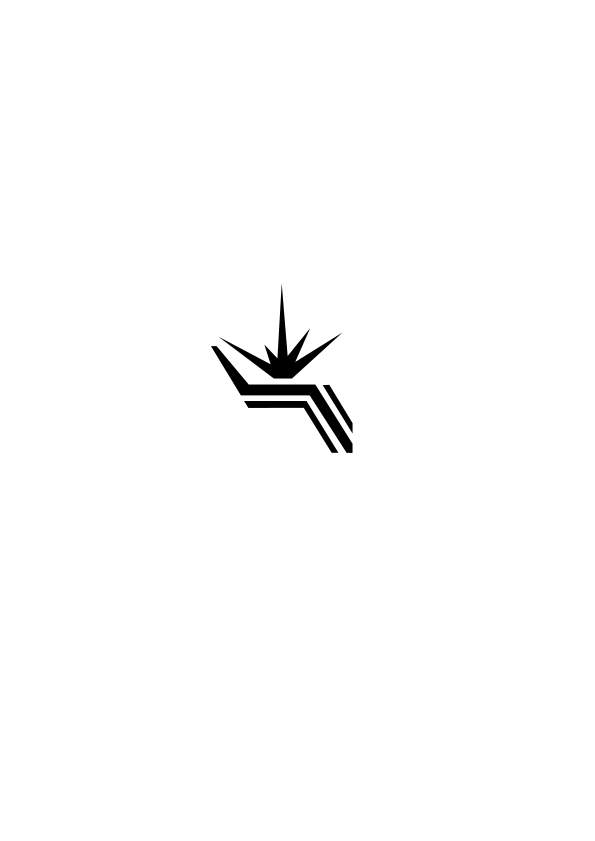
\includegraphics[width=\textwidth]{../BINP-logo}
    % \end{minipage}\hfill
    % \begin{minipage}{0.23\linewidth}
    % 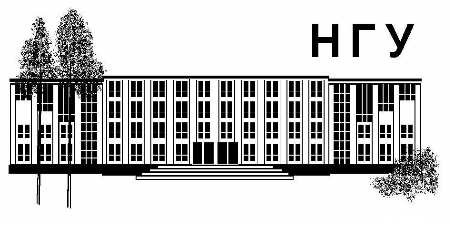
\includegraphics[width=\textwidth]{../NSU-logo}
    % \end{minipage}
    % \hfill
    % \hspace*{6em}

    
    % Кафедра теоретической физики физического факультета НГУ
    % \medskip

    % \Large
    % Профессор Грабовский А.\,В.
    % \smallskip

    % \huge
    % \textbf{Общая теория относительности}
    % \smallskip

    % \Large
    % Лекция № 10
     \vfill

     \normalsize
     \begin{minipage}{0.8\linewidth}
      Получение сохраняющихся величин в осесимметричной стационарной
      метрике. Увлечение инерциальных систем отсчета. Угловая скорость
      частицы с нулевым моментом импульса в осесимметричной
      стационарной метрике. Угловая скорость света, испущенного
      перпендикулярно радиусу при постоянном $\theta$, Предел
      статичности, поверхность бесконечного красного смещения,
      горизонт событий. Метрика Шварцшильда во входящих координатах
      Эддингтона"=Финкельштейна. Устранение координатной
      сингулярности. Диаграмма Финкельштейна для световых
      геодезических. Наклон световых конусов при $r>2M$, $r<2M$,
      $r=2M$. Сингулярности кривизны. Решение Керра. Экстремальное
      поле Керра. Асимптотика на больших расстояниях, переход в
      решение Шварцшильда при нулевом моменте вращения. Предел
      статичности, поверхность бесконечного красного смещения,
      горизонт, сингулярности. Эргосфера. Процесс Пенроуза.

     \end{minipage}
    \vfill

    \normalsize \ccbysa\hspace{0.5em}  Новосибирск 2022
  \end{center}
\end{titlepage}
\end{document}
